\documentclass[a4paper,12pt]{article}
\usepackage{setspace}
\usepackage{sectsty}
\usepackage{siunitx}
\usepackage{graphicx}
\usepackage[a4paper, total={3in, 9in}, textwidth=16cm,bottom=1in,top=1.4in]{geometry}
\usepackage[dvipsnames]{xcolor}
\usepackage{amsmath}
\usepackage{esvect}
\usepackage{soul}
\usepackage{amsthm}
\usepackage{svg}
\usepackage{hyperref}
\usepackage{longtable}
\usepackage{draftwatermark}
\usepackage{helvet}
\renewcommand{\familydefault}{\sfdefault}
\usepackage{float}
\usepackage{amssymb}
\usepackage{outlines}
\usepackage{caption}
\usepackage{fancyvrb}
\usepackage{subcaption}
\usepackage{esdiff}
\usepackage{dirtytalk}
\usepackage{colortbl}
\usepackage{booktabs}
\usepackage{setspace}
\usepackage{mathtools}
\usepackage{tikz,pgfplots}
\usepackage[most]{tcolorbox}
\usepackage{tikz-network}
\SetWatermarkText{timthedev07}
\SetWatermarkScale{4}
\SetWatermarkColor[gray]{0.97}
\usetikzlibrary{positioning,decorations.markings,arrows.meta,angles,quotes}
\DeclarePairedDelimiter{\ceil}{\lceil}{\rceil}
\newtheorem{lemma}{Lemma}
\newtheorem{proposition}{Proposition}
\newtheorem{remark}{Remark}
\newtheorem{observation}{Observation}
\doublespacing
\let\oldsection\section
\renewcommand\section{\clearpage\oldsection}
\newcommand{\RNum}[1]{\uppercase\expandafter{\romannumeral #1\relax}}
\let\oldsi\si
\renewcommand{\si}[1]{\oldsi[per-mode=reciprocal-positive-first]{#1}}
\usepackage{enumitem}
\newcommand{\subtitle}[1]{%
  \posttitle{%
    \par\end{center}
    \begin{center}\large#1\end{center}
    \vskip0.5em}%
}
\newcommand{\degsym}{^{\circ}}
\newcommand{\Mod}[1]{\ (\mathrm{mod}\ #1)}
\usepackage{hyperref}
\hypersetup{
  colorlinks=true,
  linkcolor = blue
}
\newcommand{\lb}{\\[8pt]}
\newenvironment*{cell}[1][]{\begin{tabular}[c]{@{}c@{}}}{\end{tabular}}
\newcommand{\img}[4]{\begin{center}
  \begin{figure}[H]
    \centering
    \includegraphics[width=#2\textwidth]{#1}
    \caption{#3}
    \label{fig:#4}
  \end{figure}
\end{center}}
\parindent=0pt
\usepackage{fancyhdr}
\fancyfoot{}
\fancypagestyle{fancy}{\fancyfoot[R]{\vspace*{1.5\baselineskip}\thepage}}
\renewcommand{\contentsname}{Table of Contents}
\newcommand{\angled}[1]{\langle{#1}\rangle}
\newcommand{\paren}[1]{\left(#1\right)}
\newcommand{\sqb}[1]{\left[#1\right]}
\newcommand{\coord}[3]{\angled{#1,\, #2,\, #3}}
\newcommand{\pair}[2]{\paren{#1,\, #2}}
\newcommand{\atom}[3]{{}^{#1}_{#2}\text{#3}}
\usepackage[
  noabbrev,
  capitalise,
  nameinlink,
]{cleveref}

\crefname{lemma}{Lemma}{Lemmas}
\crefname{proposition}{Proposition}{Propositions}
\crefname{remark}{Remark}{Remarks}
\crefname{observation}{Observation}{Observations}

\newtcolorbox[auto counter]{prob}[2][]{fonttitle=\bfseries, title=\strut Problem~\thetcbcounter: #2,#1,colback=Orchid!5!white,colframe=Orchid!75!black,top=5mm,bottom=5mm}

\newtcolorbox[auto counter]{rem}[1][]{fonttitle=\bfseries, title=\strut Remark.~\thetcbcounter,colback=purple!5!white,colframe=purple!65!gray,top=5mm,bottom=5mm}

\newtcolorbox[auto counter]{defin}[1][]{fonttitle=\bfseries, title=\strut Definition.~\thetcbcounter,colback=black!5!white,colframe=black!65!gray,top=5mm,bottom=5mm}

\newtcolorbox[auto counter]{obs}[1][]{fonttitle=\bfseries, title=\strut Observation.~\thetcbcounter,colback=RedViolet!5!white,colframe=RedViolet!65!gray,top=5mm,bottom=5mm}

\newtcolorbox[auto counter]{lem}[1][]{fonttitle=\bfseries, title=\strut Lemma.~\thetcbcounter,colback=Maroon!5!white,colframe=Maroon!65!gray,top=5mm,bottom=5mm}

\newtcolorbox[auto counter]{prop}[1][]{fonttitle=\bfseries, title=\strut Proposition.~\thetcbcounter,colback=RedOrange!5!white,colframe=RedOrange!65!gray,top=5mm,bottom=5mm}

\newtcolorbox[auto counter]{hint}[1][]{fonttitle=\bfseries, title=\strut Hint.~\thetcbcounter,colback=OliveGreen!5!white,colframe=OliveGreen!75!gray,top=5mm,bottom=5mm}

\setlength{\belowcaptionskip}{-20pt}
\begin{document}


\pagenumbering{arabic}
\pagestyle{fancy}


\begin{titlepage}
  \begin{center}

    \vspace*{8cm}
    \textbf{\Large {IB Physics Topic B1 Thermal Energy Transfers; SL \& HL}} \\
    \vspace*{1cm}
    \large{By timthedev07, M25 Cohort}

  \end{center}
\end{titlepage}

\pagebreak
\tableofcontents
\pagebreak

\clearpage
\setcounter{page}{1}
\addtocontents{toc}{\protect\thispagestyle{empty}}

\section{The Kelvin Scale}

The Kelvin scale is an absolute scale, where 0 K is the lowest possible temperature. The conversion to Celsius is given by
$$T(K) = T(\degsym C) + 273$$
E.g., 0 K is -273$\degsym$ C.

\section{Phases of Matter}

\begin{table}[H]
  \centering
  \begin{tabular}{|p{0.15\textwidth}|p{0.15\textwidth}|p{0.25\textwidth}|p{0.15\textwidth}|p{0.2\textwidth}|}
    \hline
    \textbf{Phase} & \textbf{Shape} & \textbf{Volume}                         & \textbf{Particular Separation} & \textbf{Compression} \\ \hline
    Solid          & Fixed          & Fixed                                   & Very close                     & Very difficult       \\ \hline
    Liquid         & Not fixed      & Fixed                                   & Close                          & Difficult            \\ \hline
    Gas            & Not fixed      & Not fixed; expand to fill the container & Far apart                      & Easy                 \\ \hline
  \end{tabular}
  \caption{Comparison of properties of the three phases of matter}
  \label{tab:phases_of_matter}
\end{table}

Many substances such as water move between the three states depending on the kinetic energy in its molecules.

\section{Temperature and Energy}

When two objects with different temperatures come in contact, eventually they will reach thermal equilibrium (both at the same temperature).\lb
All objects above 0 K possess some internal kinetic energy in its particles. The higher the temperature, the higher the average kinetic energy of the particles.

\subsection{Internal Energy}

Internal energy is defined as the sum of KE and potential, as follows
\begin{center}
  \textit{The internal energy of the system is the sum of the total potential energy arising from the intermolecular forces and the total KE of the molecules from Brownian motion.}
\end{center}
Notes on the potential energy:
\begin{itemize}
  \item The stronger the intermolecular attractive forces, the higher the potential energy.
  \item The larger the separation between particles, also the higher the potential energy. This should not be confused with the impact of the attractive force --- a stronger attraction does not necessarily mean a closer separation.
\end{itemize}


When energy is supplied to a substance, both components of the internal energy increase:
\begin{itemize}
  \item The increase in KE causes the particles to vibrate more vigorously, which increases the temperature.
  \item The increase in potential energy causes the particles to move further apart, sufficiently so for the intermolecular bonds to be broken, decreasing density.
\end{itemize}

\pagebreak

This can then help explain the phase changes of matter.
\begin{itemize}
  \item During \textbf{melting}, the potential energy increases while the KE of the particles remains constant. This means that the temperature during this period of change remains constant, and all the supplied energy is being used to break the bonds between the particles.
  \item Similarly, during \textbf{freezing} or similar phase changes, bonds are formed between the particles, and energy is released, which keeps the average KE of the particles and thus the temperature constant.
  \item Post-melting, the KE of the particles now increases, which then will increase temperature.
  \item Molecules gain enough kinetic energy to overcome all intermolecular forces. Molecules break free, becoming a gas. This is \textbf{evaporation}.
  \item Energy transfer goes primarily to potential energy until all bonds are broken.
\end{itemize}

\subsection{Average Kinetic Energy}

Planck linked the average translational KE, $E_k$ of a gas molecule to the Kelvin temperature $T$ of the gas
$$E_k = \frac{3}{2}k_BT$$
where $k_B = \dfrac{\text{gas constant}}{\text{Avogadro's constant}} = \dfrac{R}{N_A}$ is the Boltzmann constant, $1.381 \times 10^{-23} \si{\joule\per\kelvin}$.
This constant can be thought of as the conversion factor from temperature to energy. In fact, temperature is a measure of the level of KE of the particles in a substance.

\pagebreak

\subsection{Specific Heat Capacity}

The specific heat capacity of a substance is the amount of energy required to raise the temperature of 1 kg of the substance by 1 K or 1 degree Celsius (the Kelvin scale is more preferable). The equation is
$$Q = mc\Delta T$$
\begin{itemize}
  \item  $Q$ is the energy supplied to the substance in joules.
  \item $m$ is the mass of the substance in kg.
  \item $c$ is the specific heat capacity of the substance in $\si{\joule\per\kilogram\per\kelvin}$.
  \item $\Delta T$ is the change in temperature in K or $\degsym$ C.
\end{itemize}

\subsection{Specific Latent Heat}

The specific latent heat $L$ for a phase change is the amount of energy $Q$ required to change one kilogram of the substance from one phase to another. In other words,

$$L = \dfrac{Q}{m} \quad \text{ equivalently } \quad Q = mL$$

\img{phasechangegraph}{0.65}{A typical phase change graph}{phase_change_graph}

The above graph outlines how the temperature changes during a phase change.
\begin{itemize}
  \item The graph assumes that the energy is supplied at a constant rate, i.e. energy and time can be used interchangeably as the $x$-axis.
  \item The horizontal segments represent the phase change itself, where the temperature remains constant and all the supplied energy is used to break the bonds.
  \item The sloped lines represent intervals in which the temperature changes without changing the state.
  \item There are two types of specific latent heat:
        \begin{enumerate}
          \item \textbf{Specific latent heat of fusion} is used for melting and freezing, i.e. phase changes between a solid and a liquid.
          \item \textbf{Specific latent heat of vaporization} is used for boiling and condensation, i.e. phase changes between a liquid and a gas.
        \end{enumerate}
  \item \hl{The longer horizontal statements indicate a larger specific latent heat}, assuming the mass is fixed.
  \item \hl{The steeper the slope, the smaller the specific heat capacity.}
  \item Across the two ends of a horizontal segment (a phase change), the internal energy increases because
        \begin{itemize}
          \item Although the temperature and hence the average KE of the particles remains constant
          \item the potential energy increases.
        \end{itemize}
\end{itemize}

\section{Conduction}

It is an energy transfer mechanism without bulk movements of particles. There are two mechanisms of conduction:
\begin{enumerate}
  \item \textbf{Lattice vibration} in solids, the energy is transferred by the vibrations of the particles in the lattice. Through this mechanism, the particles in the hotter region transfer kinetic energy to the particles in the cooler region, hence propagating heat through the material.
  \item \textbf{Free electron movement} in metals, the free electrons carry the energy from the hotter region to the cooler region, by colliding with atoms and electrons to transfer its kinetic energy.
\end{enumerate}

Metals are good conductors of heat due to the presence of \textbf{free electrons}; this allows them to propagate heat using both mechanisms. Non-metals are poor conductors due to the lack of free electrons --- they cannot propagate heat through free electron movement.\lb
Conduction is much less important in liquids and gases, as the particles are much more spread out. In these states, convection is the primary mode of heat transfer.


\subsection{Thermal Conductivity}

\textbf{Thermal conductivity} is a measure of how well a thermal conductor can transfer thermal energy through itself in a \textit{steady state} (when the temperature at any point in the object is not changing).
$$\text{conductivity} = \frac{\text{average rate of energy transfer}}{\text{area of material}\times\text{temperature gradient}}$$

\pagebreak

$$\frac{\Delta Q}{\Delta t} = \kappa A\times \frac{\Delta T}{\Delta x}\quad \text{ or } \quad \kappa = \frac{\Delta Q}{\Delta t}\times\frac{\Delta x}{A\Delta T}$$
where
\begin{itemize}
  \item $\kappa$ is the thermal conductivity in $\si{\watt\per\meter\per\kelvin}$.
  \item $Q$ is the energy transferred in joules.
  \item $t$ is the time taken in seconds.
  \item $A$ is the cross-sectional area of the material in $\si{\meter\squared}$, relative to the direction of heat propagation.
  \item ${\Delta T}$ is the difference in K or $\degsym$ C across the two ends of the material of length $\Delta x$.
\end{itemize}

The idea of thermal conductivity can be used in the design of \textit{double-glazed windows}: The air in between the two glass panels has a poor thermal conductivity --- this reduces the rate of heat transfer between the inside and outside of the building.

\section{Convection}

A heat transfer mechanism through the movement of particles in a fluid. The particles in the hotter region move faster, becoming less dense and rise. The particles in the cooler region are denser thus sink. This creates a convection current, which transfers heat from the hotter region to the cooler region.

\subsection{Sea Breezes}

During the day, the land has a higher surface temperature than the sea; it heats up the air above it, causing the air to expand (decrease density) and rise, pulling in cooler air from the sea. The inverse happens during the night.

\begin{minipage}{0.5\textwidth}
  \img{day.png}{1.0}{Sea breeze during the day}{day}
\end{minipage}%
\begin{minipage}{0.5\textwidth}
  \img{night.png}{1.0}{Land breeze during the night}{night}
\end{minipage}%

\pagebreak

\subsection{Convection in Earth}

In some parts of the world:
\begin{enumerate}
  \item The Earth's core is hot and acts at the heat source.
  \item The mantle is a fluid, and the heat from the core causes the mantle to rise, creating an upwelling motion.
  \item Two currents operate in the same direction and drive the crust upwards, creating new land.
\end{enumerate}

In other parts
\begin{enumerate}
  \item The convection currents pull the mantle down, creating a subduction zone.
  \item This pulls the crust downwards.
\end{enumerate}

\subsection{Winds}

\begin{enumerate}
  \item The heating of the Earth's surface by the Sun is uneven.
  \item This creates areas that are hotter and areas that are cooler.
  \item In hotter areas, the air rises, creating a low-pressure zone.
  \item Conversely, in cooler areas, the air sinks, creating a high-pressure zone.
  \item Air flows from high- to low-pressure zones, creating winds.
  \item The velocity of wind interacts with the Earth's rotation, creating the Coriolis effect.
  \item This leads to the rotation of the air masses such that the air circulates in a clockwise direction in the northern hemisphere and anti-clockwise in the southern hemisphere.
\end{enumerate}

\pagebreak

\subsection{Hot Air Balloons}

\begin{enumerate}
  \item The air in the canopy is heated by a burner.
  \item The temperature of the air increase, decreasing its density.
  \item This creates a density difference between the hot air in the balloon and the cooler air outside.
  \item Due to the pressure difference, the balloon experiences an upthrust.
\end{enumerate}

\subsection{Minimizing Convection Current}

For instance, covering the liquid surface of a cup of hot drink with a layer of foam reduces the rate of heat loss.
\begin{enumerate}
  \item Conduction is reduced; foam traps air, which is a poor conductor.
  \item Convection current is reduced; the upper surface of the foam is cooler, and this reduces the temperature difference with the surrounding air, thus, minimizing the convection current.
\end{enumerate}


\section{Thermal Radiation}

This is the transfer of thermal energy through electromagnetic radiation. This means that the transfer does not require a medium, and can occur in a vacuum. The energy is transferred in the form of photons, which are massless particles that travel at the speed of light.\lb
When ions accelerate, they emit electromagnetic radiation. This is the basis of thermal radiation.\lb
Matt black surfaces are good emitters and absorbers of radiation, while shiny surfaces are poor absorbers and emitters but good reflectors.

\section{Black Body Radiation}

A \textbf{black body} is a perfect emitter and absorber of radiation that absorbs E.M. radiation of all wavelengths that are incident on it. This is an idealized concept that cannot be realized in practice. However, a good approximation is a small hole in a cavity, where the radiation is absorbed and re-emitted multiple times, thus approximating a black body.
\begin{itemize}
  \item \textbf{Perfect absorption}: When radiation enters the small hole, it has very little chance of escaping. The radiation bounces around inside the cavity, reflecting multiple times off the walls. With each reflection, some of the energy is absorbed by the cavity walls. Eventually, nearly all the incident radiation will be absorbed.
\end{itemize}
The following are true for the emission of radiation from the cavity:
\begin{enumerate}
  \item The intensity of radiation is independent of the material from which the cavity is made.
  \item The intensity increases with increasing temperature.
\end{enumerate}

\subsection{The Emission Spectrum}

Light consists of different wavelengths, and the intensity of radiation emitted at different wavelengths is called the emission spectrum. This can be measured by a spectrometer.\lb
A spectrometer measures the intensity of radiation emitted for each of the different wavelengths that the radiation encapsulates.\lb
Intensity, in $\si{\W\per\m\squared}$, is given as the power emitted per unit area
$$I = \frac{P}{A}$$

The following graph is one obtained from the spectrometer:

\begin{minipage}{0.45\textwidth}
  \img{spectrumgraph.png}{1}{Sun's spectrum, assuming it's a black-body}{spectrum}
\end{minipage}%
\hspace{0.1\textwidth}
\begin{minipage}{0.5\textwidth}
  \img{spectragraphs.png}{1}{Black-body spectra for
    other temperatures}{spectra}
\end{minipage}

\cref{fig:spectrum} shows the following
\begin{itemize}
  \item There is a peak value at around $\SI{500}{\nano\m}$
  \item The intensity is greater in the visible region than in the invisible region.
  \item Towards the positive infinity direction on the $x$-axis, the intensity decreases, infinitely tending to zero.
\end{itemize}

The family of curves in \cref{fig:spectra} shows that, as temperature increases
\begin{itemize}
  \item the overall intensity of radiation increases
  \item the curves skew towards shorter wavelengths; the peaks translate towards the origin.
\end{itemize}

\pagebreak

\subsection{Wien's Displacement Law}

This states that the wavelength at which the intensity of radiation is maximum $\lambda_{\max}$ is related to the absolute temperature of the black body $T$ by
$$\lambda_{\max}T = b$$
where $b$ is Wien's displacement constant, $2.9 \times 10^{-3} \si{\m\kelvin}$. This should not be confused with the apparent brightness of an object.\lb
This equation allows us to predict the peak wavelength of the radiation emitted by a black body at a given temperature.

\subsection{Stefan-Boltzmann Law}

This states that the total power (total energy radiated per second), equivalently, the luminosity $L$ emitted by a black body is given by
$$P \equiv L = \sigma A T^4$$
\begin{itemize}
  \item $A$ is the total surface area of the black body.
  \item $\sigma$ is the Stefan-Boltzmann constant, $5.67 \times 10^{-8} \si{\W\per\m\squared\per\kelvin\tothe{4}}$.
  \item $T$ is the temperature of the black body in K.
\end{itemize}

Note that this equation is often combined with \cref{eq:brightness}.\lb
Also note that the Stefan-Boltzmann law \textbf{only considers heat transfer by radiation} and thus does not account for conduction or convection. Hence, the realistic rate of transfer is higher than the calculated value, as convection and conduction also take place.

\pagebreak

\subsection{Observational Astronomy}

\begin{figure}[H]
  \centering
  \includesvg[width=0.5\textwidth]{Inverse_square_law}
\end{figure}

The intensity $I$ of radiation decreases with distance $d$ from the source and it obeys the inverse square law. The following provides an intuitive explanation:
\begin{itemize}
  \item At $d = 1$, the intensity is $I$, and the total energy is distributed over an area of $A$.
  \item At $d = 2$, the area over which the energy is distributed is $4A$ (by considering scale factors). However, the total energy is the same, but now it is distributed over four times the original, which means that the energy per unit area is $\dfrac{1}{4}$ of the original.
\end{itemize}

Formally, the relationship is given by
\begin{equation}\label{eq:intensity}
  I = \frac{P}{4\pi d^2}
\end{equation}
where $P$ is the total power emitted by the source and $I$ is measured in $\si{\W\per\m\squared}$


\subsection{Apparent Brightness}

The apparent brightness $b$ of a star is just the intensity of radiation received from the star at the Earth's surface. This is given by the following, which is analogous to \cref{eq:intensity}
\begin{equation}\label{eq:brightness}
  b = \frac{L}{4\pi d^2}
\end{equation}
where $L \equiv P$ is the luminosity of the star, and $d$ is the star-Earth distance.

\pagebreak

\section{Exam Questions}

\subsection{Intensity Wavelength Curve}

\img{ex/1.png}{0.9}{Graph}{ex1}

\img{ex/2.png}{0.9}{Options}{ex2}

\begin{itemize}
  \item There are two things to find out about
        \begin{enumerate}
          \item Whether the peak wavelength is shifted: We invoke Wien's displacement law $$\lambda_{\max}T = b$$
                and see that with a lower temperature, the peak wavelength is greater and so the peak will shift to the right.

          \item Whether the intensity is greater or less: We invoke the intensity equation $$I = \sigma T^4$$ and deduce that a lower temperature means a lower intensity. This means that the peak will be lower.
        \end{enumerate}
  \item Combining the two findings, we obtain that \textcolor{ForestGreen}{the answer is A}.
\end{itemize}

\pagebreak

\subsection{Misc \#1}

The star $\delta$ Vel A is a main sequence star that has a black-body spectrum as shown.

\img{ex/3.png}{0.9}{Graph}{ex3}

\begin{enumerate}[label=(\alph*)]
  \item Show that the surface temperature of $\delta$ Vel A is about 9000 K.
        \begin{itemize}
          \item We read off the graph that the peak wavelength is roughly $\lambda_{\max} = 3.0 \times 10^{-7} \si{\m}$.
                \begin{align*}
                  T = \frac{b}{\lambda_{\max}} = \frac{2.9 \times 10^{-3} \si{\m\kelvin}}{3.0 \times 10^{-7} \si{\m}} = 9350 \si{\kelvin}
                \end{align*}
        \end{itemize}
  \item The apparent brightness of $\delta$ Vel A is $\SI{2.2e-9}{\W\per\m\squared}$ and it is $\SI{6.2e14}{\km}$ from Earth. Estimate the radius of $\delta$ Vel A.

        \begin{itemize}
          \item Here we relate the two equations involving luminosity \begin{align*}
                  L = \sigma A T^4 \quad & \text{ and } \quad b = \frac{L}{4\pi d^2} \\
                  \sigma(4\pi R^2)T^4    & = 4\pi b d^2                              \\
                  \sigma R^2 T^4         & = bd^2                                    \\
                  R                      & = \sqrt{\frac{bd^2}{\sigma T^4}}          \\
                                         & = \SI{1.4}{\giga\m}
                \end{align*}
        \end{itemize}
  \item The radius of the Sun, $R_\odot$, is $\SI{7e5}{\km}$. Sketch, on the Hertzsprung-Russell diagram, the position of $\delta$ Vel A.
        \img{ex/4.png}{0.7}{Hertzsprung-Russell diagram}{ex4}
        \begin{itemize}
          \item $R_\delta \approx 2R_\odot$.
          \item Any point within the specified area is acceptable.
        \end{itemize}
\end{enumerate}

\pagebreak

\subsection{Equilibrium Temperature \#1}

Small pieces of solid paraffin with a total mass of 30 g at a temperature of 42 °C are mixed with 150 g of liquid paraffin at a temperature of 240 °C. The mixture is stirred until an equilibrium temperature is reached.

The following data for paraffin are available:

\begin{itemize}
  \item Specific heat capacity of solid paraffin $c_\text{solid} = \SI{0.7}{\kilo\joule\per\kilogram\per\kelvin}$
  \item Specific heat capacity of liquid paraffin = $c_\text{liquid} = \SI{2.13}{\kilo\joule\per\kilogram\per\kelvin}$
  \item Specific latent heat of fusion of paraffin = $L = \SI{220}{\kilo\joule\per\kilogram}$
  \item Melting point of paraffin = 47 °C
\end{itemize}

\begin{enumerate}[label=(\alph*)]
  \item Calculate the theoretical equilibrium temperature of the mixture.
        \begin{itemize}
          \item First things first, we must be clear that the solid paraffin will melt and so in its calculation we have to take into account both the latent heat and the specific heat capacity. This however not the case for the liquid paraffin, as there is no clue in the question that it will freeze or boil.
          \item We form the following equation -- the LHS is original solid, which will heat up, melt, and then heat up again (three stages). The RHS is the liquid paraffin, which will cool down (one stage only). Let us denote $T$ as the equilibrium temperature and we shall proceed to solve for it.
                \begin{align*}
                  Q_{\text{heating up to melting point}} + Q_{\text{melting}} + Q_{\text{heating liquid}}                               & = Q_{\text{cooling liquid}}                           \\
                  m_\text{solid}c_\text{solid}(T_\text{melt} - 42) + m_\text{solid}L + m_\text{solid}c_\text{liquid}(T - T_\text{melt}) & = m_\text{liquid}c_\text{liquid}(T_\text{liquid} - T) \\
                \end{align*}
                Solving this gives $T = \SI{190}{\degreeCelsius}$.
        \end{itemize}
  \item When the experiment was carried out, the equilibrium temperature of the mixture was found to be different from the theoretical value. Suggest the reason for this difference.
        \begin{itemize}
          \item The heat loss to the surroundings is not taken into account in the theoretical calculation.
          \item This means that the theoretical equilibrium is higher than the actual value.
        \end{itemize}
  \item The mixture was held in a large metal container during the mixing. Explain \textbf{one} change to the procedure that will reduce the difference in (b).
        \begin{itemize}
          \item Insulate the container OR
          \item Carry out experiment quicker OR
          \item Use larger volumes of substances
        \end{itemize}
\end{enumerate}

\pagebreak

\subsection{Thermal Conductivity -- Ratios}

Window 1 is made of a single glass pane of thickness $d$. Window 2 is made of two glass panes of thickness $d$ each, separated by a thin airspace. Both windows have the same surface area and separate air masses of the same temperature difference.

Thermal energy transferred in unit time through window 1 is $Q$. The thermal energy transferred in unit time through window 2 is

\begin{enumerate}[label=\Alph*.]
  \item Less than $\dfrac{Q}{2}$.
  \item Equal to $\dfrac{Q}{2}$.
  \item Between $\dfrac{Q}{2}$ and $Q$.
  \item Equal to $2Q$.
\end{enumerate}

\begin{itemize}
  \item We invoke the equation for thermal conductivity
        $$\frac{\Delta Q}{\Delta t} = \kappa A\times \frac{\Delta T}{\Delta x}$$
        and see that the rate of energy transfer is inversely proportional to the thickness of the material. In this case, the thickness is at least doubled for window 2, and so the rate of energy transfer is halved at least.
  \item We then need to consider the function of the air space: Air is a good insulator and that further reduces the heat transfer. Hence, \textcolor{ForestGreen}{A is the correct answer}.
\end{itemize}

\pagebreak

\subsection{Air, Ice, and Water}

A layer of ice on the surface of a lake separates cold air from relatively warmer unfrozen water.

The temperature of the air and the temperature of the water can both be assumed constant. The thickness of the ice gradually increases. What effect does the change in ice thickness have on the temperature gradient across the ice and the rate of thermal energy transfer by conduction through the ice?

\begin{itemize}
  \item The temperature gradient $\dfrac{\Delta T}{\Delta x}$ is decreased: The temperature difference across the two ends is the difference between the temperatures of the water and the air, which is constant. The thickness $\Delta x$ of the ice increases, and so the temperature gradient decreases.
  \item As a result, the rate of thermal energy transfer by conduction through the ice decreases, since $\dfrac{\Delta Q}{\Delta t} = \kappa A\times \dfrac{\Delta T}{\Delta x}$.

\end{itemize}

\pagebreak

\subsection{Thermal Conduction \#1}

A sealed bottle contains 0.50 kg of water at an initial temperature of 60 °C. The bottle is made of glass of thickness 3.0 mm and thermal conductivity $\SI{0.90}{\W\per\m\per\kelvin}$.

\begin{enumerate}[label=(\alph*)]
  \item The temperature of the air outside of the bottle is 20 °C. The surface area of the bottle is $\SI{4.0e-2}{\m\squared}$. Calculate the initial rate of thermal energy transfer by conduction through the bottle.
        \begin{align*}
          \frac{\Delta Q}{\Delta t} & = \kappa A\times \frac{\Delta T}{\Delta x}                            \\
                                    & = 0.9 \times (\SI{4.0e-2}{})\times \frac{60 - 20}{3.0 \times 10^{-3}} \\
                                    & = \SI{480}{\W}
        \end{align*}
  \item Explain why the rate calculated in part (a) is decreasing.
        \begin{itemize}
          \item The rate of energy transfer is directly proportional to the temperature difference across the two ends of the material.
          \item As the water cools down, the temperature difference decreases, and so does the rate of energy transfer.
        \end{itemize}
  \item Estimate the initial rate of the change of the temperature of the water in the bottle. State your answer in $\si{\K\per\s}$. The specific heat capacity of water is $\SI{4200}{\joule\per\kilogram\per\kelvin}$.
        \begin{align*}
          Q = mc\Delta T     & \implies P = \diff{Q}{t} = mc\diff{\Delta T}{t}     \\
          480                & = 0.5 \times 4200 \times \diff{\Delta T}{t}         \\
          \diff{\Delta T}{t} & = \frac{480}{0.5 \times 4200} = \SI{0.23}{\K\per\s}
        \end{align*}
\end{enumerate}

\pagebreak

\subsection{Conduction or Convection?}

The ends of a vertical column of water are maintained at different temperatures $T_t$ and $T_b$ both above the freezing point.

\img{ex/5.png}{0.2}{Column of water}{ex5}

Energy transfer by radiation in this arrangement is negligible.

\begin{enumerate}[label=(\alph*)]
  \item Discuss the mechanism that accounts for the greatest rate of energy transfer when:
        \begin{enumerate}[label=(\roman*)]
          \item $T_t > T_b$.
                \begin{itemize}
                  \item Conduction
                  \item Energy transfers through interaction of particles in liquid at atomic scale
                \end{itemize}
          \item $T_t < T_b$.
                \begin{itemize}
                  \item Convection
                  \item Energy transfers through movement of bodies of liquid at different densities, namely the hotter and less dense regions rise, while the cooler and denser regions sink.
                \end{itemize}
        \end{enumerate}
  \item The liquid now freezes so that the vertical column is entirely of ice. Suggest how your answer to (a)(ii) will change.\begin{itemize}
          \item Now, the solid cannot move relative to material above it
          \item So conduction only
        \end{itemize}
\end{enumerate}


\subsection{Ideally Lagged vs. Unlagged Rod}

A rod is formed from two metal rods XY and YZ of identical dimensions. End X and end Z are at different temperatures.

\img{ex/6.png}{0.5}{Rod}{ex6}


The side of the rod can be unlagged or ideally lagged. Explain the difference in energy transfer for these two cases.

\begin{itemize}
  \item When ideally lagged, no energy transfer can occur through the sides of the bar.
  \item All the power input/ energy input persecond at one end will emerge at the other end.
  \item When unlagged, energy transfer occurs from the sides of the bar and the power at input $>$ power output at the other end.
\end{itemize}

\pagebreak

\subsection{Heat Propagation through Cubes -- Ratios}

A metal cube X of length $L$ is heated gaining thermal energy $Q$. Its temperature rises by $\Delta T$. A second cube Y, of length $2L$, made of the same material, gains thermal energy of $2Q$. What is the temperature rise of Y?

\begin{itemize}
  \item We know that the temperature rise is such that
        $$\Delta T \propto \frac{Q}{m}$$
  \item For the second cube, the doubled length means that the mass is $8m$.
  \item The energy gained is $2Q$.
  \item Altogether, this gives a down-scaling factor of $\frac{1}{4}$, thus $$\frac{\Delta T}{4}$$
\end{itemize}

\pagebreak

\subsection{Two Blocks in Contact}

Two blocks X and Y at different temperatures are placed in thermal contact with each other until they reach thermal equilibrium. Block X and block Y are
of the same material. The mass of block Y is half that of block X. The change in temperature of block X has a magnitude $\Delta T$ and the change in internal energy
of block X has a magnitude $\Delta U$. What is the change in magnitude of temperature of block Y and the change in magnitude of internal energy of block Y?

\img{ex/7.png}{0.5}{Options}{ex7}

\begin{itemize}
  \item First, we must establish that the energy transferred \textbf{away from} the block that is hotter is equal to the energy transferred \textbf{to} the cooler block. Already, this \textcolor{red}{eliminates options A and B}.
  \item Now, let's invoke the equation $\Delta Q = mc\Delta T$ and equate $\Delta Q_X = \Delta Q_Y$; knowing that they are of the same material, we can cancel out s.h.c.
        \begin{align*}
          m_X\Delta T_X & = m_Y\Delta T_Y            \\
          m_X\Delta T   & = \frac{1}{2}m_X\Delta T_Y \\
          T_Y           & = 2\Delta T_X
        \end{align*}
        This leads us to the \textcolor{ForestGreen}{answer D}. The important step is to invoke precisely $\Delta Q = mc\Delta T$ and not the conductivity equation, the key reason being that we have no knowledge of the area of contact.
\end{itemize}

\pagebreak

\subsection{Hard MCQ -- Equilibrium of Mixtures}

Three samples of the same liquid are mixed in an insulated container.The masses and initial temperatures of the samples are:

\begin{table}[H]
  \centering
  \begin{tabular}{|c|c|c|}
    \hline
    \textbf{Sample} & \textbf{Mass} & \textbf{Initial temperature (°C)} \\ \hline
    A               & $2M$          & 60                                \\ \hline
    B               & $2M$          & 30                                \\ \hline
    C               & $M$           & 0                                 \\ \hline
  \end{tabular}
  \caption{Samples of liquid}
  \label{tab:liquid_samples}
\end{table}

What is the equilibrium temperature of the mixture?

\begin{itemize}
  \item Although this may not be immediately obvious, but the concerned formula in this question is
        $$Q = mc\Delta T$$
  \item Now, if it were only for a two sample mixture, it would be much easier since the energy transfer from one equals the energy transfer to the other. However, in this case, we have three samples and so we need to be careful.
  \item We must first sort out the directions of energy transfer. Consider the following diagram, where the bigger nodes represent higher initial temperatures:
        \begin{figure}[H]
          \centering

          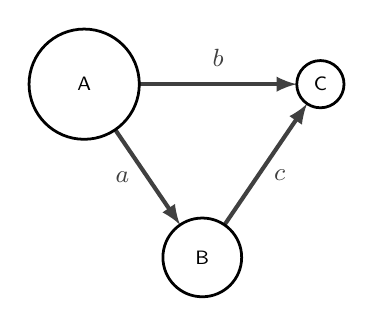
\begin{tikzpicture}
            \Vertex[color=none,label=A,size=1.4]{A}
            \Vertex[color=none,x=1.5,y=-2.2,label=B,size=1]{B}
            \Vertex[color=none,x=3,label=C,size=.6]{C}
            \Edge[label=$a$,fontsize=\small,position={left=5pt},Direct](A)(B)
            \Edge[label=$b$,fontsize=\small,position={above=5pt},Direct](A)(C)
            \Edge[label=$c$,fontsize=\small,position={right=5pt,below},Direct](B)(C)

          \end{tikzpicture}
        \end{figure}
  \item It is constructed on the principle that heat flows from the hotter to the cooler without external work done.
  \item Let the equilibrium temperature be $T_0$, then, we can obtain the following equations, each relating the change in temperature and the energy transfer of a single sample:
        \begin{align*}
          -a-b & \equiv 2M(T_0 - 60) \\
          a-c  & \equiv 2M(T_0 - 30) \\
          b+c  & \equiv M(T_0)
        \end{align*}
        We have cancelled out the specific heat capacity, since they are all the same.

        The important bit of these equations is consistency in the signs
        \begin{itemize}
          \item On the right-hand side, all temperature changes are in the form of $T_0 - T_i$.
          \item On the left-hand side, transfers of a negative sign indicate a loss of energy, and vice versa.
        \end{itemize}

  \item Solving for $T_0$ gives $T_0 = 36$.
  \item Phew, lovely question.

\end{itemize}

\pagebreak

\subsection{Moles and Molar Masses in a Mixture}

A vessel contains a mixture of helium and methane gas. 40\% of the mass of the gas is composed of helium, with the rest composed of methane.

If there is a total of 11 moles of gas in the vessel, what is the number of moles of methane in the gas?

\[
  \text{Molar mass of helium} = 4 \, \text{g mol}^{-1}
\]
\[
  \text{Molar mass of methane} = 16 \, \text{g mol}^{-1}
\]

\begin{itemize}
  \item Let $N_H$ be the number of moles of helium and $N_M$ be the number of moles of methane.
  \item We know that $N_H + N_M = 11$.
  \item We also know that the mass ratio of $M_H$ : $M_M$ is 4 : 6.
        \begin{align*}
          \text{Mass of helium}  & = N_H \times 4  \\
          \text{Mass of methane} & = N_M \times 16 \\
          \frac{4N_H}{16N_M}     & = \frac{4}{6}   \\
          \frac{N_H}{4N_M}       & = \frac{2}{3}   \\
          3N_H                   & = 8N_M          \\
        \end{align*}
  \item We know have a system of equations, if we multiply the first equation of the sum of the molecules by 3 and substitute the second one in, we obtain $N_M = 3$.
\end{itemize}

\end{document}